\documentclass[../documentation.tex]{subfiles}
 
\begin{document}
\section{Alkalmazáshoz szükséges műszaki feltételek elemzése}
\subsection{Projekt részletes leírása}
A projekt célja egy olyan robot demo hardveres és szoftveres kidolgozása, amely képes egy emberrel (továbbfejlesztés után akár egy másik robottal) lejátszani egy sakkjátszmát. A demo az ember-robot kollaboráció bemutatására szolgál, fontos szempont az interakció biztonságos megvalósítása mind az emberre, mind a környező tárgyakra tekintettel.\\

A megvalósításhoz a következő problémák megoldására van szükség:
\begin{enumerate}
	\item szükséges biztonsági funkciók beüzemelése,
	\item a bábuk helyzetének felismerése az egyes lépések előtt és után,
	\item a bábuk megfogása és mozgatása (ide tartozik a kalibráció és a referenciafelvétel),
	\item sakkalgoritmus beágyazása a programba,
	\item a sakkbábúk és a tábla megtervezése és megvalósítása,
	\item jelzés a robotkar számára, ha lépés történt.
\end{enumerate}
A felsorolt pontok a projekt során következőképpen kerültek kidolgozásra:
\begin{itemize}
	\item A bábuk helyzetének detektálása a projekt során QR-kód kereső és olvasó képfeldogozó eljárásokon alapul (a bábuk tetején található a kód). A kamera a roboton kerül rögzítésre.
	\item A bábuk mozgatása egy elektromosan vezérelt, párhuzamos megfogó (\angol{gripper}) segítségével történik.
	\item Ahhoz hogy a bábuk megfogása egyszerű legyen, azonos magasságú és azonos módszerrel megfogható bábuk készülnek.
	\item A biztonsági funkciók főként az tengelyekben ébredő plusz nyomatékok monitorozására és biztonsági zónák definiálására épül.
	\item A tábla és a robotkar, illetve a megfogó (egy jól definiált pontja) és a robotkar relatív helyzetének kalibrálására a robotvezérlő szoftverben elérhető alapfunkciók kerültek felhasználásra.
	\item A sakklépés megtörténtétét a robotvezérlőhöz kötött külső gombbal tudja a felhasználó jelezni.
	\item A képek fogadása, feldolgozása és a sakkalgoritmus futtatása mind a robotvezérlőn történik.
	\item Mivel a robotvezérlőn Java alapú környezet fut magas szinten, így a képfeldolgozó és a sakkozó programok is ebben lettek implementálva.
\end{itemize}

\subsection{A megfogó vezérlése}
\subsubsection{A vezérlés hardveres kialakítása}
Ahhoz hogy a megfogót (grippert) a robotvezérlőn futó programból lehessen irányítani több kiegészítő eszközre is szükség van a gripperen és a vezérlőegységén kívül. Többféle konstrukcióval is el lehet érni ezt a célt; a projekt során használt összeállítás elemei (\ref{fig:grippersetup}):
\begin{itemize}
	\item \textbf{Megfogó (gripper):} párhuzamosan mozgó, két pofájú, elektromos megfogó; pontos típusa: SCHUNK MEG 50 EC\cite{grippermanual}.
	\item \textbf{Grippervezérlő:} a megfogóhoz tervezett vezérlő; pontos típusa: SCHUNK Controller MEG EC\cite{grippermanual}
	\item \textbf{Analóg és digitális I/O modulok\footnote{I/O (\angol{(Input/Output)}: bemeneti és kimeneti modulok}:} a robotvezérlő ezen modulok segítségével tudja irányítani a grippervezérlőt. A felhasznált eszközök Beckhoff gyártmányúak. Pontos tipusaik:
	\begin{itemize}
		\item EL1809: 16 csatornás, digitális bemeneti modul\footnote{https://www.beckhoff.com/english.asp?ethercat/el1809.htm}
		\item EL2809: 16 csatornás, digitális kimeneti modul\footnote{https://www.beckhoff.com/english.asp?ethercat/el2809.htm}
		\item EL3002: 2 csatornás, analóg bemeneti modul\footnote{https://www.beckhoff.hu/english.asp?ethercat/el3002.htm}
		\item EL4032: 2 csatornás, analóg kimeneti modul\footnote{https://www.beckhoff.com/english.asp?ethercat/el4032.htm}
	\end{itemize}
	\item \textbf{EtherCAT\footnote{Általános ismertető az EtherCAT-ről: https://en.wikipedia.org/wiki/EtherCAT} Coupler:} az I/O modulok az ú.n. E-bus-on keresztül kommunikálnak. Ahhoz hogy a robotvezérlőhöz lehessen kötni az E-bus-t, EtherCAT Coupler-re van szükség. Pontos tipusa: Beckhoff EK1100\footnote{https://www.beckhoff.com/english.asp?ethercat/ek1100.htm}.
	\item \textbf{Tápegység:} a fentebb felsorolt eszközök mindegyike 24 V megtáplálást igényel, ezt a projekt során egy Siemens tápegység szolgáltatja.
\end{itemize}

\begin{figure}
\centering
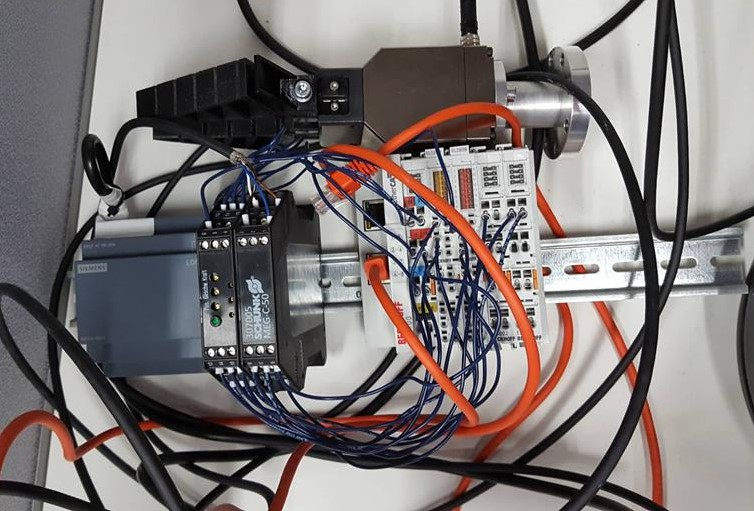
\includegraphics[scale=0.75]{grippersetup}
\caption{Kép a megfogóhoz tartozó konstrukcióról}
\label{fig:grippersetup}
\end{figure}

\subsubsection{A megfogó szoftveres konfigurációja}
KUKA SunriseOS esetén (és általánosságban a KUKA robotok esetén) a különböző bemeneti, kimeneti és kommunikációs csatornák kezelésére I/O konfigurációs fájl generálására van szükség. Ezeket a fájlokat a WorkVisual nevű program segítségével lehet létrehozni és szerkeszteni. Adott SunriseOS-hez meghatározott a kompatibilis Sunrise Workbench verzió (ebben a programban a legegyszerűbb a robotvezérlőn futó program megírása, feltöltése). Adott Sunrise Workbench verzóval kompatibilis WorkVisual verzóra vonatkozó információkat a Sunrise Workbench-et megnyitva a Help->Sunrise.OS Release Notes menüpont alatt találunk. A szakdolgozathoz felhasznált szoftverek és környezet:
\begin{itemize}
	\item SunriseOS 16
	\item Work Visual 5.0.5 build600
	\item Windows 10 a PC-n
\end{itemize}

A megfelelő IOConfig elkészítéséhez az alábbi lépések szükségesek:
\begin{enumerate}
	\item Ahhoz hogy a WorkVisual verziót összekössük a Sunrise Workbench-csel importálni kell a Workbench-hez tartozó Sunrise.kop fájl a WorkVisual-ba. Ez a fájl a telepített Workbench verzióhoz tartozó mappán belül a `WorkVisual AddOn' nevű almappában található. Az importálás menete: WorkVisual->Extras->Option package management->Install... gomb. A felugró ablakban lehet kiválasztani a megfelelő Sunrise.kop fájlt és telepíteni. Ahhoz hogy az egyes Beckhoff modulokkal lehessen kommunikálni szükség van a `Device description file'-ok importálására. Ezek a fájlok a gyártó oldaláról letölthetőek\footnote{Device description files: https://www.beckhoff.com/english.asp?download/elconfg.htm}. A (XML) fájlok importálásához a WorkVisual->Import / Export->Import device description file lehetőséget kell választani (ezt a műveletet adott eszközön csak egyszer kell elvégezni, új projekt esetén ezt a lépést már ki lehet hagyni). A megfelelő fájlok kiválasztása és importálása után szükség van a DTM Catalog frissítésére (WV->Extras->DTM Catalog Management->Search for installed DTMs). A fájlok használatához a `Known DTMs' részről át kell emelni az elemeket a `Current DTM Catalog' részre (\ref{fig:dtmcatalog}).
	\item A Sunrise Workbench-ben új projekt létrehozása után a projektre jobb egérgomb->New->I/O Configuration. A WorkVisual automatikusan elindul. A projektre jobb egérgombbal kattintva (WV-ban) a `\angol{Set as active controller}' lehetőséget kell választani. A busz struktúrákhoz hozzá kell adni a `KUKA Extension Bus (SYS-X44)' elemet ahhoz, hogy az EtherCAT kommunikációt inicializáljuk a robotvezérlőben. Ehhez adhatjuk hozzá az EK1100 EtherCAT Coupler-t, ami az összeköttetést biztosítja a robotvezérlőben található EtherCAT hálózat és a modulok között (E-bus). Az egyes modulokat ehhez adhatjuk hozzá a programban. \textbf{Fontos:} az egyes fájlokat olyan sorrendben kell hozzáadni, ahogy azok fizikailag kapcsolódnak egymáshoz (\ref{fig:ethercatconfig} ábra).
	\item Ahhoz hogy ezeket a be- és kimeneteket a Sunrise Workbench-ben használni tudjuk szükség van Sunrise I/O Group létrehozására (VW->IO Mapping->Sunrise I/Os->Creates signals at the provider). Az I/O Group-nak tetszőleges nevet adhatunk. Az egyes be- és kimenetek kezeléséhez létrehozhatunk változókat az I/O Group-on belül. A gripper nyitásához és zárásához alapvetően 3 változó deklarálása elegendő\footnote{A gripper nyitásához és zárásához elegendő csak a digitális ki- és bementeket használni, de például a pozíció követéséhez használni kell analóg bemeneti modult, a fogóerő programból történő beállításához pedig analóg kimeneti modult.}), pl.:
	\begin{itemize}
		\item OpenGripper: bool, output, digital
		\item CloseGripper: bool, output, digital
		\item Status: bool, input, digital
	\end{itemize}
Az egyes változókat a kívánt bemenetekkel és kimenetekkel \angol{Drag and drop} módszerrel lehet összerendelni (\ref{fig:signalsmatching}). Megfelelő összekötés esetén a változók mellletti szürke nyilak zölddé változnak.
	\item Az elkészült I/O konfigurációt exportálni kell ahhoz, hogy a Sunrise Workbench-ben használni lehessen (WV->File->Import / Export->\angol{Export I/O Configuration to Sunrise Workbench project}). A Workbench-ben ezek után megjelenik az `src' mappában egy ioAccess nevű csomag. Ezen belül található az IO Group-hoz tartozó osztály (pl.: GripperContolIOGroup.java). Ez tartalmazza a szükséges methódusokat a gripper vezérléséhez, ezeket lehet meghívni a programból.
\end{enumerate}

\begin{figure}[p]
\centering
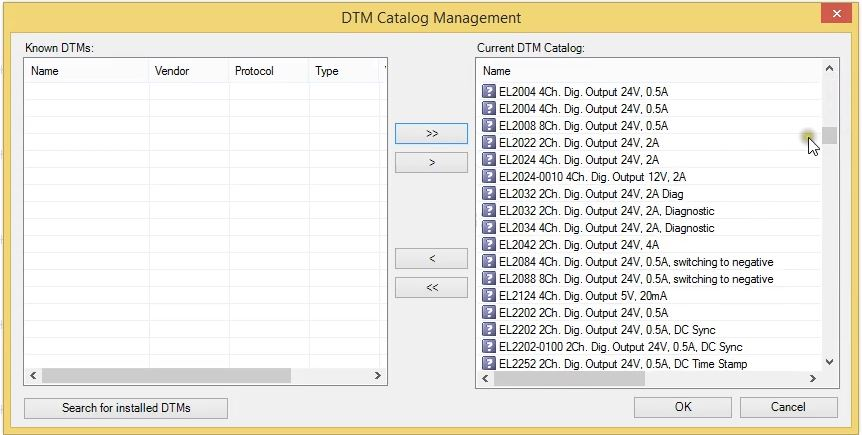
\includegraphics[scale=1]{dtmcatalog}
\caption{Az xml fájlok sikeres beimportálása után láthatjuk a \angol{Device description} fájlokat}
\label{fig:dtmcatalog}
\end{figure}

\begin{figure}[p]
\centering
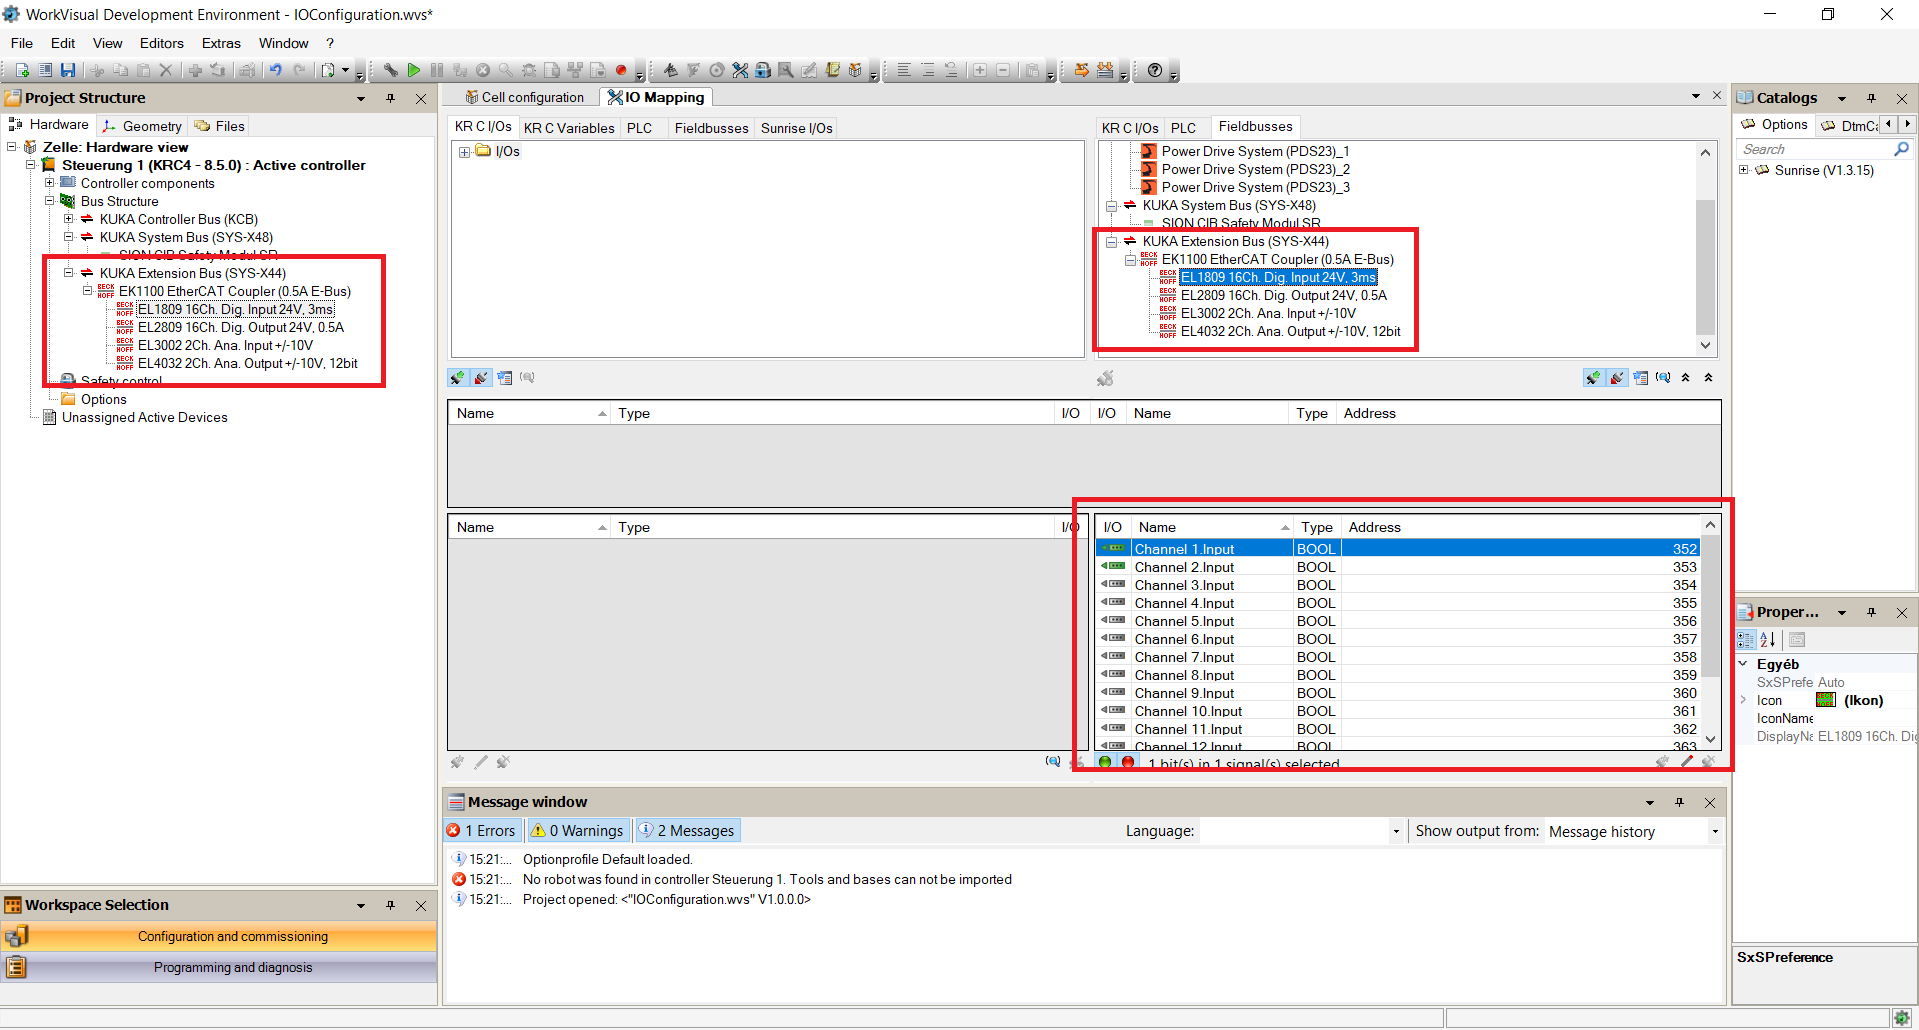
\includegraphics[scale=0.45]{ethercatconfig}
\caption{Az EtherCAT konfiguráció}
\label{fig:ethercatconfig}
\end{figure}

\begin{figure}[p]
\centering
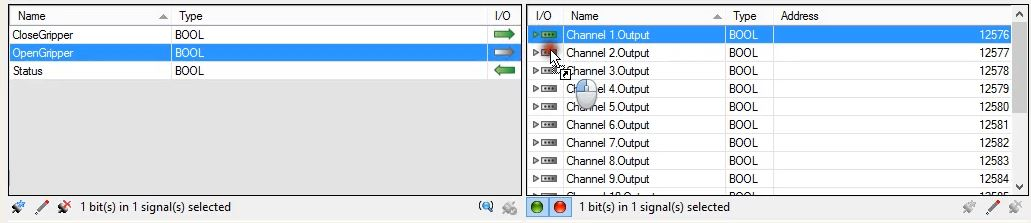
\includegraphics[scale=0.7]{signalsmatching}
\caption{Az I/O változók hozzárendelése a be- és kimenetekhez}
\label{fig:signalsmatching}
\end{figure}

\subsection{Sakkbábúk kialakítása, felismerése a képeken}
A sakkprogram működtetéséhez elegendő a bábúk új pozíciójának felismerése azután, miután az ember lépett. Elég csak az ember bábuit figyelni (a robot vezeti magának a bábuk pillanatnyi helyzetét). A sakkbábúk felismerére többfajta módszer is megfelelő lehet. A képfeldolgozást lehet saját vagy szabványos mintára alapozni (pl.: QR-kód alapú felismerés - \ref{qrsection} fejezet), illetve színes kamerakép esetén adott színek keresésére. A szakdolozat során a második módszer került beágyazásra, viszont a sakkbábuk formai kialakításakor a QR-kód alapú felismerhetőség is fontos szempont volt, így biztosítva az ilyen irányú továbbfejlesztés lehetőségét.

\subsubsection{A sakkbábuk formatervezése}
Ahhoz hogy a megfogó fel tudja emelni a bábukat könnyebség, ha a bábuk egyforma magasak, vagy ha a megfogó mindegyik bábut egy kitültetett, egy magasságban lévő részénél fogja meg (akár a talprészénél vagy alá is nyúlhatna). A talprésznél megfogás jó megoldás lehet, ha maguk a bábuk színesek, és így biztosított a képeken való felismerhetőségük. A QR-kódos továbbfejlesztéshez viszont elkerülhetetlen, hogy a QR-kód a bábuk tetején legyen elhelyezve. Ezen megfontolások alapján a bábuk végleges konstrukciója (\ref{fig:chesspieces} ábra):
\begin{itemize}
	\item Mindegyik bábu tetején található egy négyzet alapú, szélességéhez viszonyítva alacsony hasáb, amire az adott színt/színeket/QR-kódot rá lehet ragasztani.
	\item Ennél a hasábnál fogva emeli meg a megfogó a bűbut, így kevésbé kell lenyúlnia a robotkarnak, kisebb az esély arra, hogy egy másik bábut felborít.
	\item A hasáb 6 mm vastag, hogy a megfogó viszonylag nagy terhelését (min. 50 N) elviselje.
	\item Mindegyik bábu egyforma magas (40 mm), így a robotkarral felemelés programja és a képfeldolgozás is nagy mértékben leegyszerűsödik.
	\item A bábuk viszonylag alacsonyak és a talprészük vastagított, tömör, hogy kevésbé legyenek borulékonyak.
	\item Annak érdekében, hogy a bábukat kevesebb támaszanyag felhasználásával lehessen nyomtatni a bábuk tetején elhelyezkedő hasábok külön lettek kinyomtatva és csak utólag lettek a bábukra felragasztva.
\end{itemize}

\begin{figure}
\centering
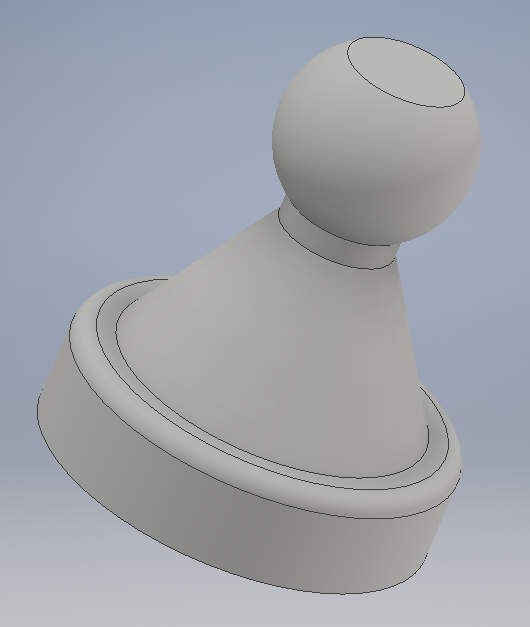
\includegraphics[height=5cm]{chess-images/pawn}
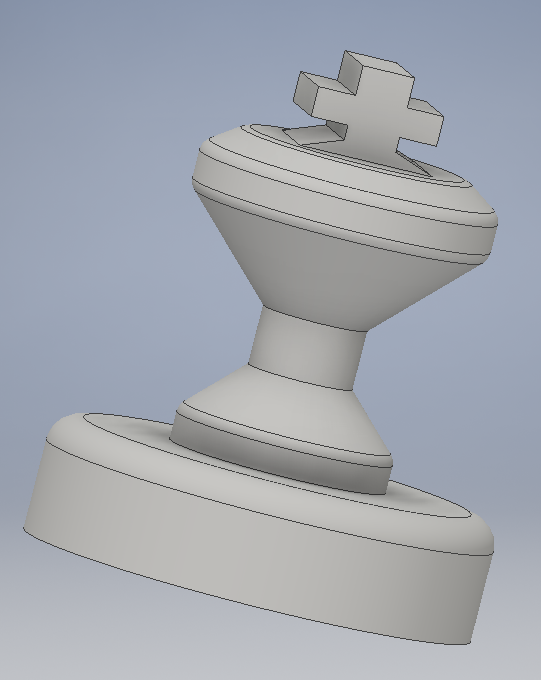
\includegraphics[height=5cm]{chess-images/king}
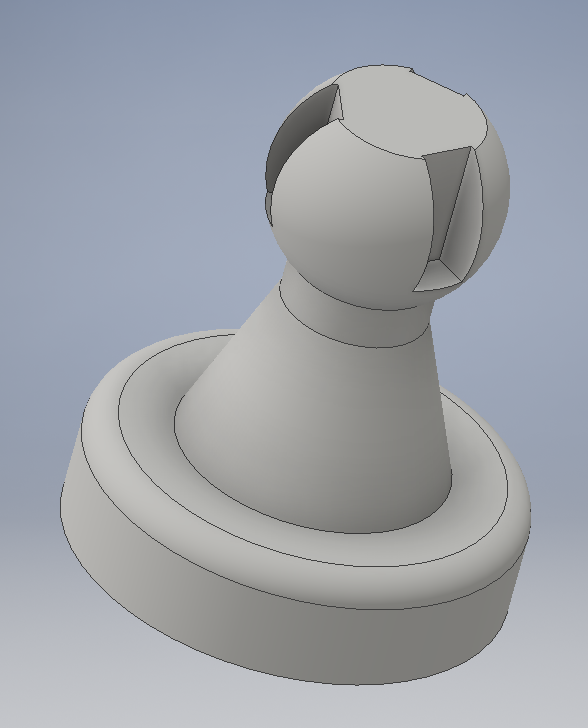
\includegraphics[height=5cm]{chess-images/bishop}
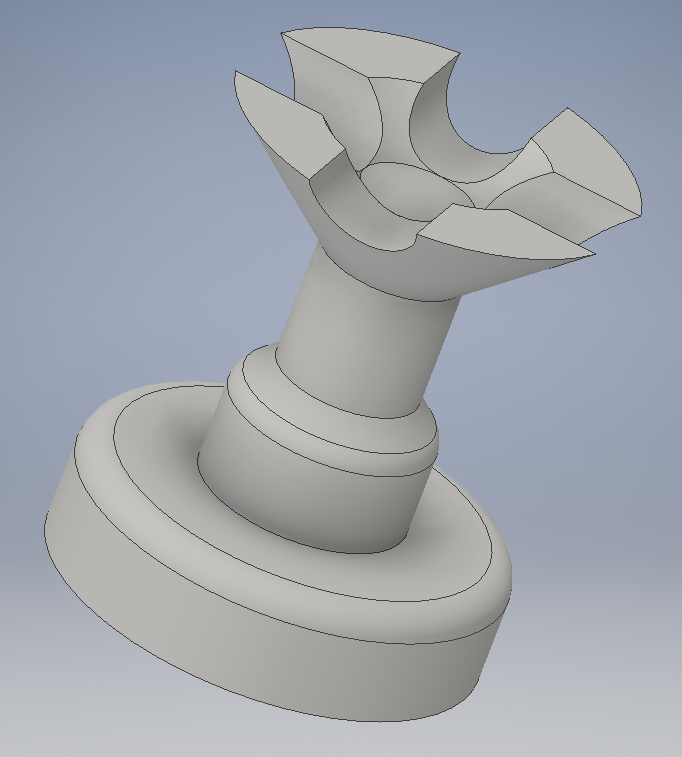
\includegraphics[height=5cm]{chess-images/queen}
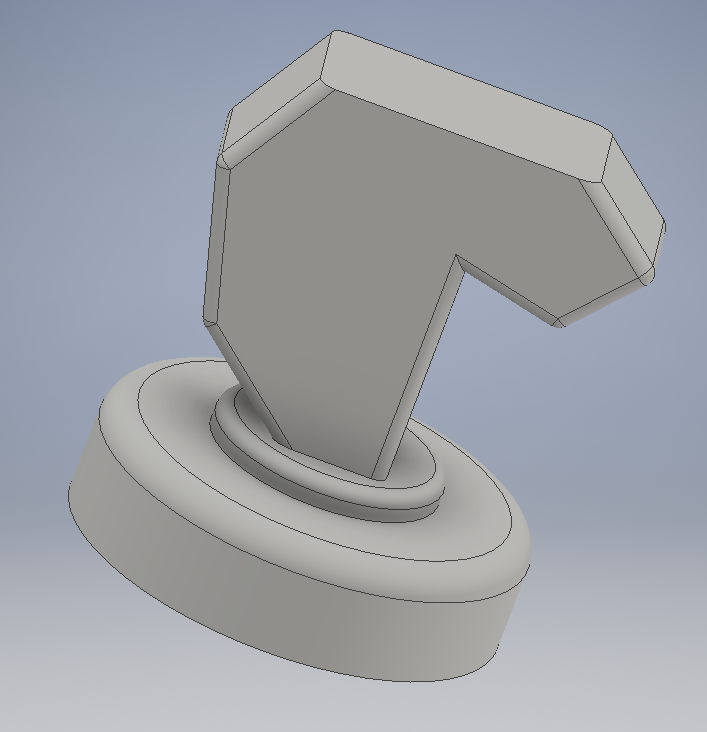
\includegraphics[height=5cm]{chess-images/knight}
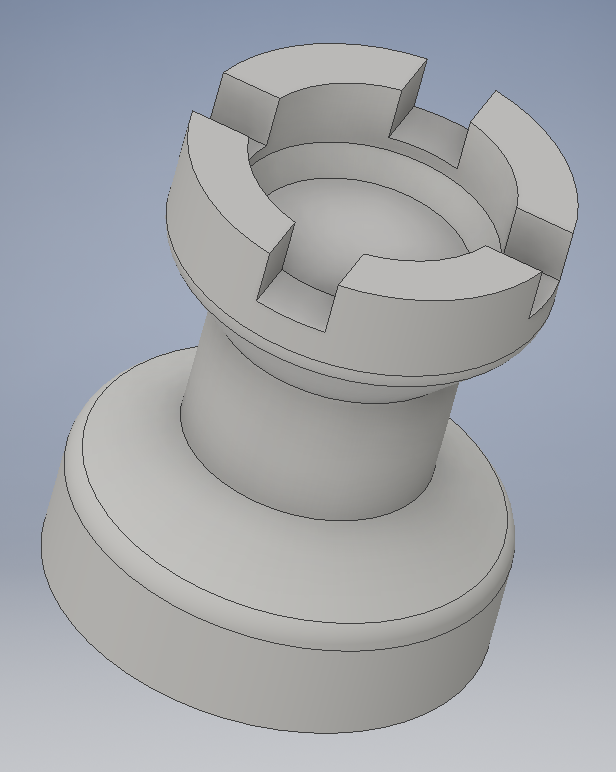
\includegraphics[height=5cm]{chess-images/rook}
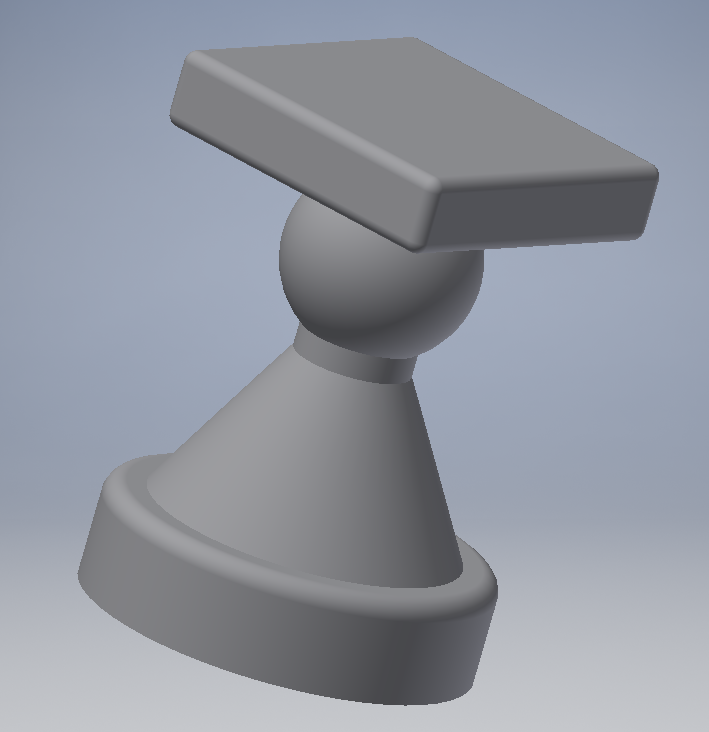
\includegraphics[height=4.8cm]{chess-images/pawnassembly}
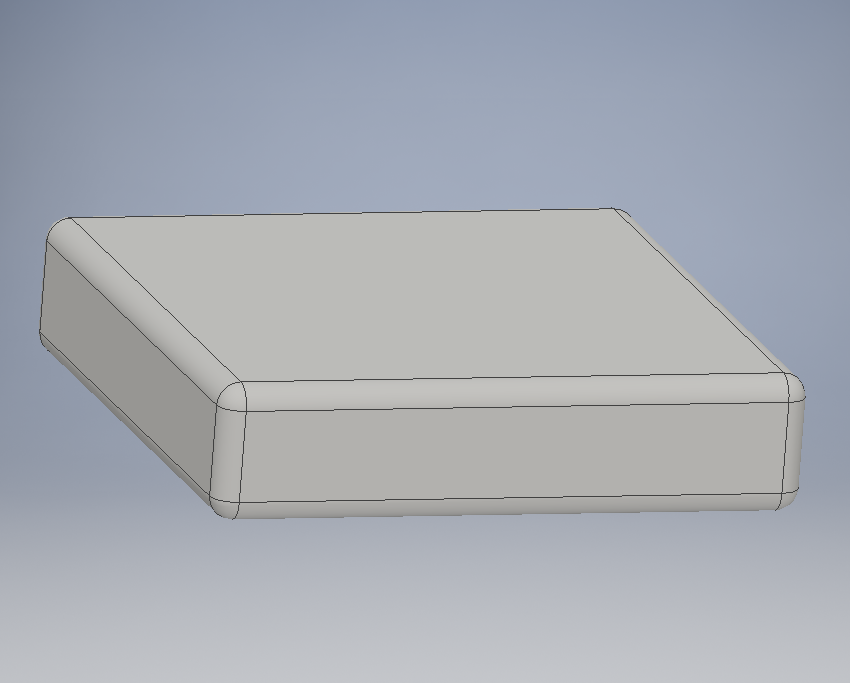
\includegraphics[height=4.8cm]{chess-images/toppart}
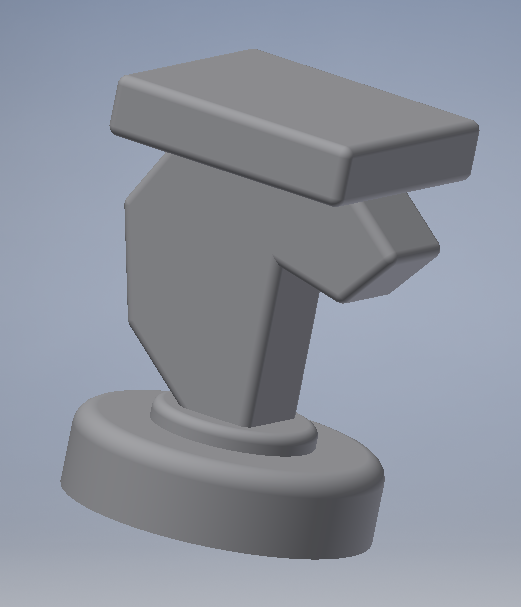
\includegraphics[height=4.8cm]{chess-images/knightassembly}
\caption{A sakkbábúk 3D-s terve}
\label{fig:chesspieces}
\end{figure}

\begin{figure}
\centering
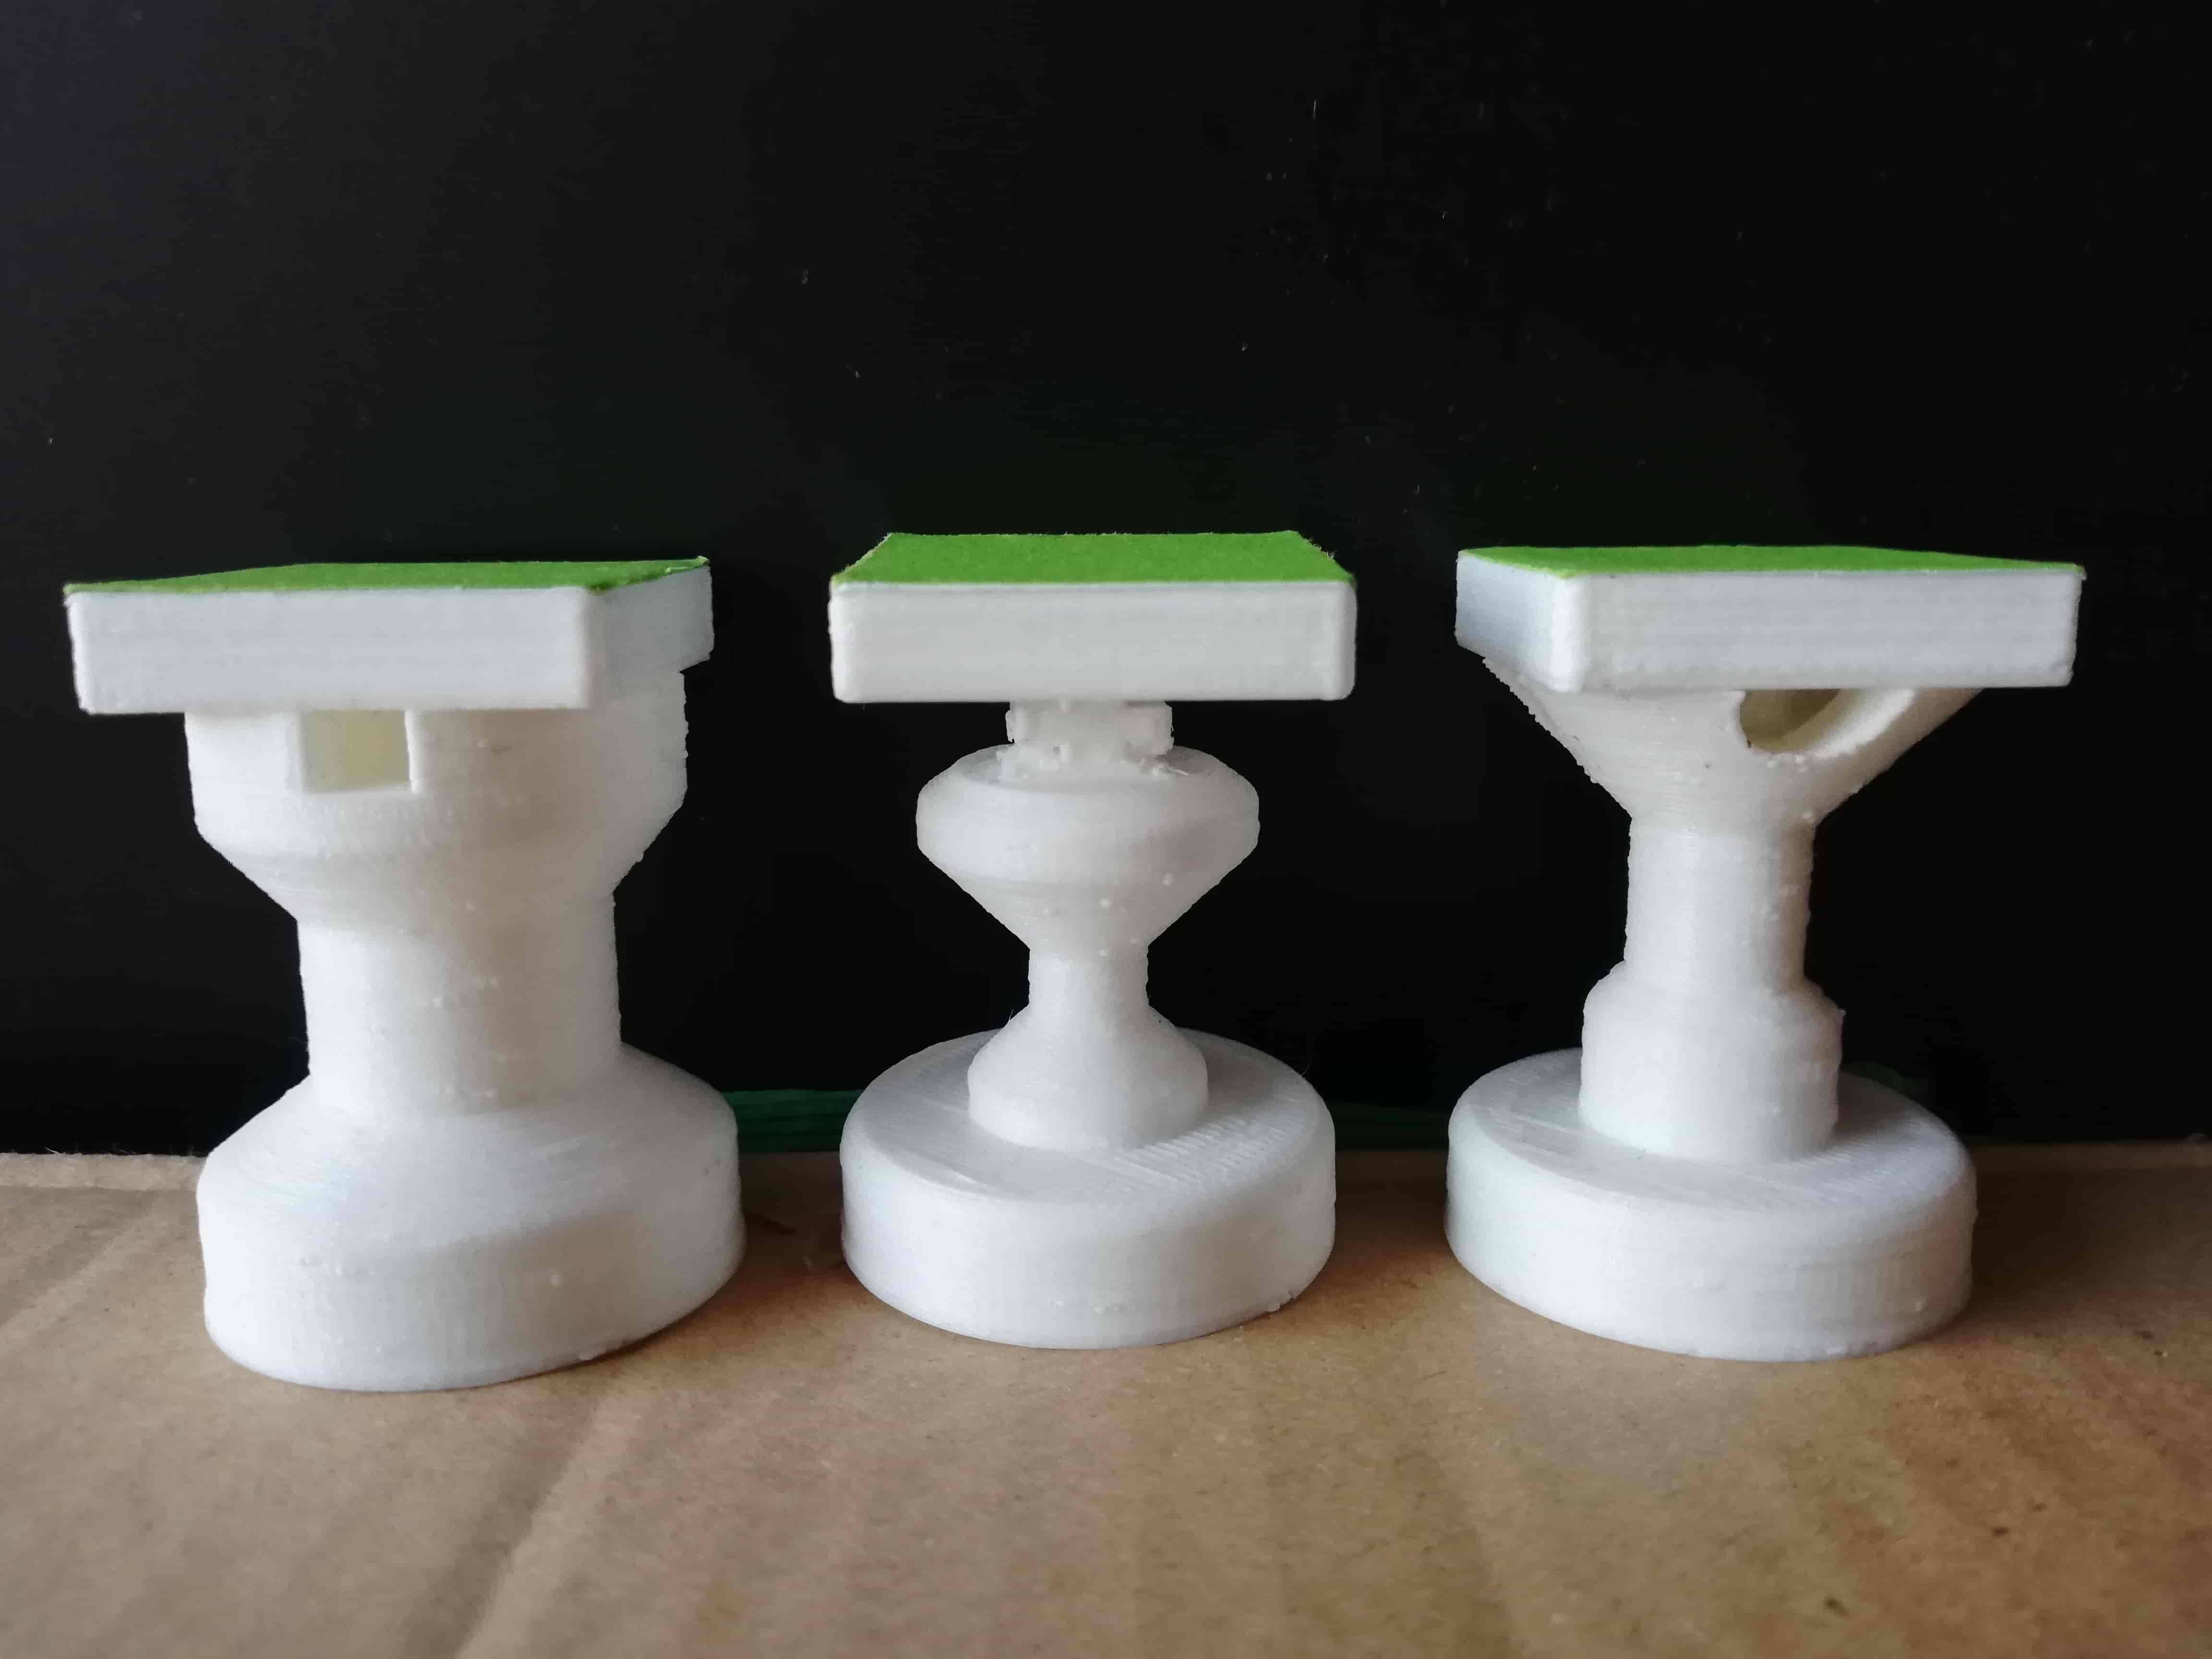
\includegraphics[scale=0.07]{chess-images/3Dprinted-min}
\caption{A kinyomtatott sakkbábuk}
\label{fig:3dprinted}
\end{figure}

\subsubsection{Bábuk pozíciójának azonosítása}

\begin{figure}[h]
\centering
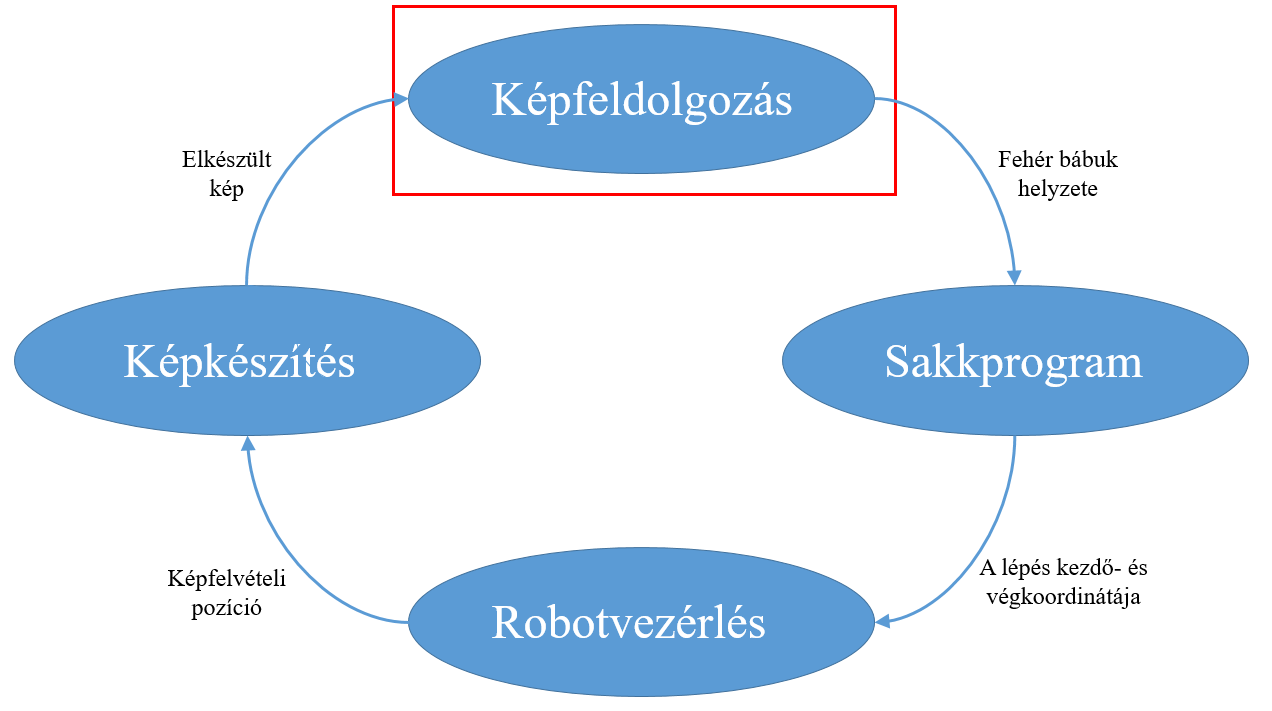
\includegraphics[scale=0.45]{flowchart-imgprocess}
\caption{A képfeldolgozás helye a folyamatban}
\label{fig:flowchart-imgprocess}
\end{figure}

A bábuk pozíciójának azonosításához szükség van valamilyen kalibrációs eljárásra, hogy a képek egyes részeihez a sakktábla mezőit tudjuk rendelni. A mezők definiálásához kötődő módszer alapjait OpenCV-s függvények jelentik. A kidolgozott eljárás lényege, hogy a kalibrációs képen egy sakktáblaminta belső sarokpontjait (azon sarokpontok, amelyek 4 mezőnek együttes sarokpontjai) határozza meg a képen. A képkoordináták alapján történik az egyes mezők felosztása az élek mentén szomszédos pontok képzeletbeli összekötésével. Mivel a perspektivikus hatások elhanyagolhatók a tábla mezőre nézve, így 2 szemközti pontra illesztett téglalap jó közelítés és az egyes képek kivágásához. Fontos elem, hogy a kalibrációs sakkminta mezőszámai vízszintes és függőleges irányban különbözzenek, mert így fogja a sarokpontkereső függvény mindig ugyanabban a sorrendben visszaadni a pontok koordinátáját. A sorszámozás a minta \underline{bal felső} részénél lévő, \underline{fekete} mező sarkától indul és soronként halad (a hosszabb élek mentén) \aref{fig:chessboardcorners} ábrán látható módon\footnote{http://stadatum.blogspot.com/2016/05/corner-identification-in-computer.html}. Az algoritmus az elmosódásokra, nagyobb szögekre (50-70°) és a papír gyűrődéseire nem érzékeny.

Fontos elem ezeken túl, hogy a kalibrációs lap abban a síkban helyezkedjen el, ahol a bábukon a zöld minta, így biztos megfelelő helyen keressük a bábukat. Ha az alsó tábla szintjére helyeznénk a kalibrációs lapot, akkor az egyes mezőkre helyezett bábukon lévő minták átlóghatnának a szomszédos mezőkre. Ezt mutatja be \aref{fig:chessboardcalibration} ábra.
Ezek alapján a kalibrációs eljárás lépései:
\begin{figure}
\centering
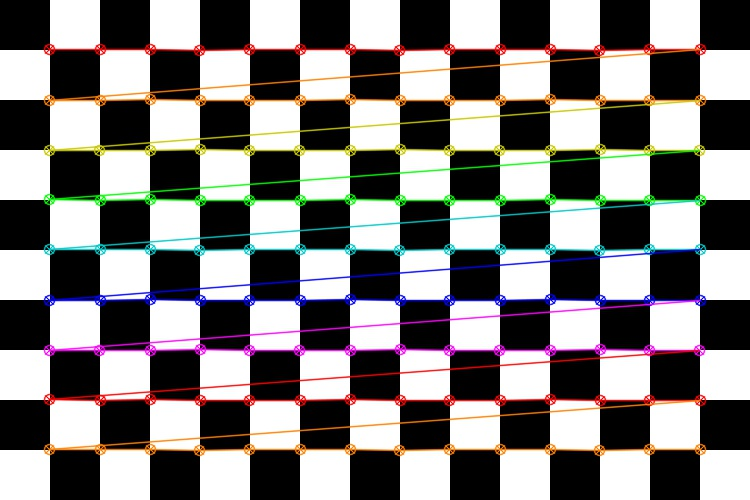
\includegraphics[scale=0.45]{chessboardcorners}
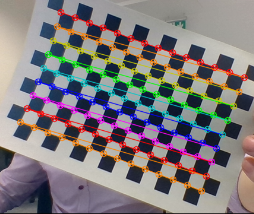
\includegraphics[scale=0.96]{chessboardcorners1}
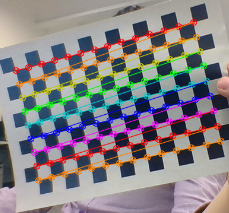
\includegraphics[scale=0.96]{chessboardcorners2}
\caption{A sakktáblaminta feltérképezett pontjai}
\label{fig:chessboardcorners}
\end{figure}
\begin{figure}
\centering
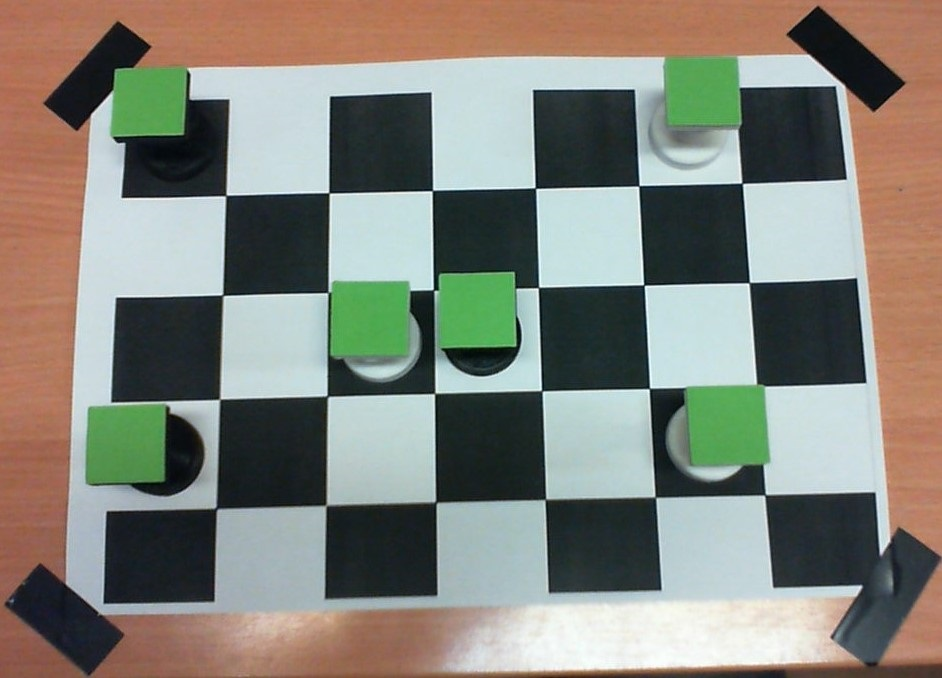
\includegraphics[scale=0.3]{beforemove}
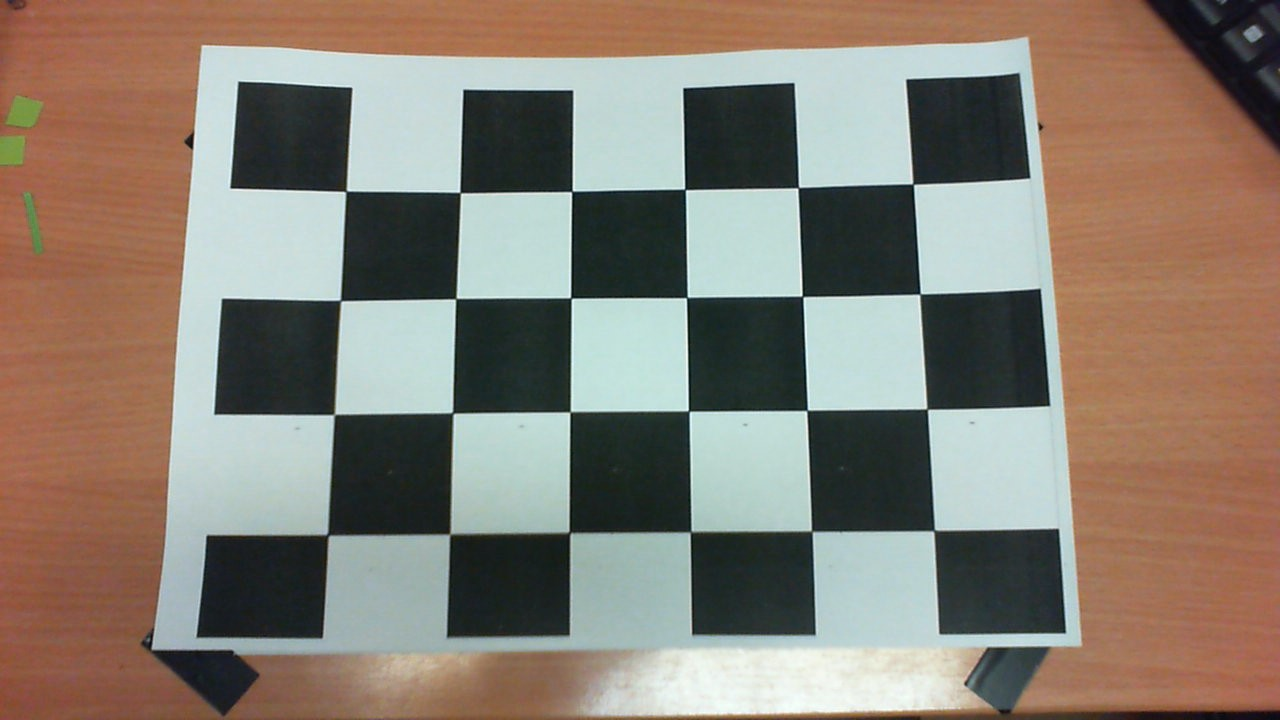
\includegraphics[scale=0.3]{calibration}
\caption{Kalibrációs kép felvétele}
\label{fig:chessboardcalibration}
\end{figure}
\begin{enumerate}
	\item Néhány sakkbábú táblára helyezése.
	\item A bábuk teteje által kifeszített síkra egy sakktáblamintás papír ráhelyezése úgy, hogy az egyes mezők az alsó sakktábla mezői felett legyenek (mindegyik alsó sakktáblamező felett legyen egy belső sarokpontokkal határolt mező).
	\item Kép készítése abból a pozícióból és szögből, ahova a robotkat a kamerával minden képkészítés előtt vissza fog térni.
	\item A képen a sarokpontok keresése és a mezők meghatározása automatikusan történik a programban, de a sarokpontok számát vízszintes és függőleges irányban előre definiálni kell.
\end{enumerate}

A képfeldolgozáshoz szükséges osztályokat az `imgprocess' csomag tartalmazza (az OpenCV-s és a QR-kódhoz tartozó .jar fájlokat a \angol{Build path}-hoz hozzá kell még adni). A sakkbábuk pozíciójának felismerését végző metódusok a ScanPiecesPosition osztályban vannak implementálva. Az osztályt példányosítani a (BufferedImage) kalibrációs képpel lehet, megadva még a horizontális és vertikális sarokpontok számát függvényparaméterként. A példányosítás hatására lefut a sarokpontkereső függvény. A ScanPosition függvényt erre a példányra meghívva visszakapjuk a fehér bábuk helyét egy boolean mátrix formájában, ahol a mátrix egyes elemei a tábla egyes mezői. A kép mezőkre darabolását a CropImages privát függvény végzi, amely a kalibráció során meghatározott sarokpontok alapján darabolja fel a képet: a kapott képek a mezők bal felső és jobb alsó pontjai által meghatározott téglalapon belüli részek.

A kapott képekről a FindGreen függvény dönti el, hogy található-e rajtuk jelentősebb kiterjedésű zöld szín. A zöld színre szűrést RGB színtartományban vizsgálja a program (HSV színskálába transzformálással a szűrés még finomítható és kevésbé lesz érzékeny a különböző fényviszonyokra is). Az egyes képek minden pixele esetén kiszámol a program egy értéket a következő képlet alapján:
\[value = greenComponent - \dfrac{redComponent}{2}  - \dfrac{blueComponent}{2}\]
Ha ez a `\angol{value}' érték egy megadott határértéknél nagyobb (jelenleg 40 egy 0-tól 255-ig terjedő skálán), akkor a pixel színét a szűrő algoritmus fehérre állítja, ellenkező esetben feketére. Utolsó lépésként a szűrő algoritmus minden mezőre külön-külön kiszámítja a fehér és a fekete pixelek számának az arányát. Ha ez az érték 10\%-nál nagyobb egy mező esetén, akkor ott található bábu, azaz a hozzá tartozó boolean mátrix elem \angol{true} értékű lesz. A visszaadott mátrixot a sakkprogram kapja majd meg, ami ez alapján és az előző állás alapján dönti el, hogy mi volt a lépés.

\begin{figure}
	\begin{subfigure}{.5\textwidth}
		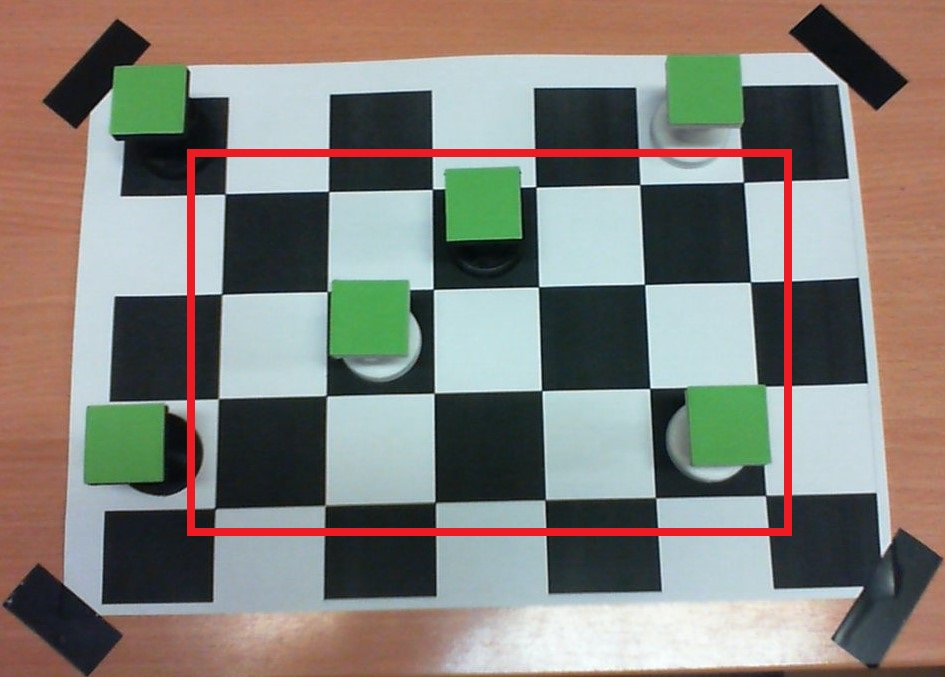
\includegraphics[scale=0.3]{imagefilter/image2filter}
		\caption{A feldolgozandó kép}
	\end{subfigure}
	\begin{subfigure}{.5\textwidth}
		\centering
		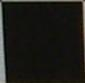
\includegraphics[width=13mm, height=13mm]{imagefilter/image0_0}
		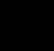
\includegraphics[width=13mm, height=13mm]{imagefilter/image0_1}
		
\includegraphics[width=13mm, height=13mm]{imagefilter/image0_2}
		
\includegraphics[width=13mm, height=13mm]{imagefilter/image0_3}
		
\includegraphics[width=13mm, height=13mm]{imagefilter/image0_4}
		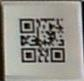
\includegraphics[width=13mm, height=13mm]{imagefilter/image1_0}
		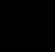
\includegraphics[width=13mm, height=13mm]{imagefilter/image1_1}
		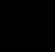
\includegraphics[width=13mm, height=13mm]{imagefilter/image1_2}
		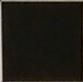
\includegraphics[width=13mm, height=13mm]{imagefilter/image1_3}
		
\includegraphics[width=13mm, height=13mm]{imagefilter/image1_4}
		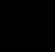
\includegraphics[width=13mm, height=13mm]{imagefilter/image2_0}
		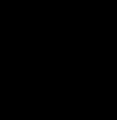
\includegraphics[width=13mm, height=13mm]{imagefilter/image2_1}
		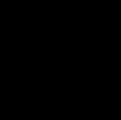
\includegraphics[width=13mm, height=13mm]{imagefilter/image2_2}
		
\includegraphics[width=13mm, height=13mm]{imagefilter/image2_3}
		
\includegraphics[width=13mm, height=13mm]{imagefilter/image2_4}
		\caption{A zöld színre szűrés eredményeként kapott képek}
	\end{subfigure}
\caption{Zöld színre szűrés (a bal oldali képen a pirossal bekeretezett rész lett kalibrálva, azokat a mezőket vizsgálja)}
\label{fig:colorfiltering}
\end{figure}

\subsection{QR-kód alapú képfeldolgozás - továbbfejlesztési irány} \label{qrsection}
Ahhoz, hogy sakkjátékot tetszőleges állapotból lehessen kezdeni, illetve folytatni szükség van a bábuk helyének felismerésén túl azok típusának egyértelmű felismerésére. Erre alkamas megoldás lehet a bábuk tetejére helyzett QR-kód, amelyben kódolva van a bábu típusa. A QR-kódok kezelésére jó választás a nyílt forráskódú ZXing (``\angol{Zebra Crossing}'') program\footnote{További információk és forráskód: https://github.com/zxing/zxing}. Ez a Java könyvtár (\angol{library}) alkamas különböző formátumú, egy- és kétdimenziós vonalkódokkal kapcsolatos képfeldolgozásra, amelynek csak egyik eleme a QR-kód olvasás és generálás.

\subsubsection{A forráskód build-je}
A könyvtár egyszerű használatához célszerű .jar fájlokat generálni a forráskódból. Az első lépés a Github-on elérhető forráskód letöltése vagy klónozása a saját számítógépre. A programkód számos mappába és almappába van rendszerezve az egyes moduloknak megfelelően (pl.: core/ és javase/). \textbf{Fontos:} a mapparendszert olyan helyre tegyük a számítógépen, melynek elérési útjában nem található szóköz karakter (ékezetes karakter is probléma lehet)! Minden Java alapú modul esetén található egy pom.xml fájl, amit Apache Maven\footnote{Az Apache Maven program ingyenesen letölthető: https://maven.apache.org/} segítségével lehet használni.

Szükségünk van megfelelő java verzió telepítésére. A JRE (\angol{Java Runtime Environment}) helyett a JDK (\angol{Java Developement Kit}) valamelyik verzióját (a projekt jdk 10.0.2 verziót használ) érdemes telepíteni, ha fejlesztői funkciókat is igénybe szeretnénk venni (a JRE csomagot ez már tartalmazza). Az Apache Maven telepítése után szükségünk van az ehhez és a JDK-hoz tartozó környezeti változók beállítására. Ezt a Vezérlőpult->Rendszer->Speciális rendszerbeállítások->Környezeti változók...->Rendszerváltozók címszó alatt tehetjük meg. Szükségünk van egy `JAVA\_HOME' és egy `M2\_HOME' változóra (\ref{fig:envvar}. ábra).

Parancssorban navigáljunk a ZXing projekt gyökeréhez és futtassuk a `mvn install' parancsot a fordításhoz, a tesztekhez és az összes modul felépítéséhez. A ``-DskipTests'' paraméter hozzáadásával a unit teszteket kihagyhatjuk. Szükség lehet a `-Drat.ignoreErrors=true' paraméterre a licensz tesztekkel kapcsolatos problémák ignorálásához. A build folyamat akkor mondható sikeresnek, ha mindegyik modul felépítése sikeres (`ANDROID\_HOME' környezeti változó beállítása nélkül az Androidhoz kapcsolódó modulokat nem build-eli) (\ref{fig:buildsuccess}. ábra).

\begin{figure}[h]
\centering
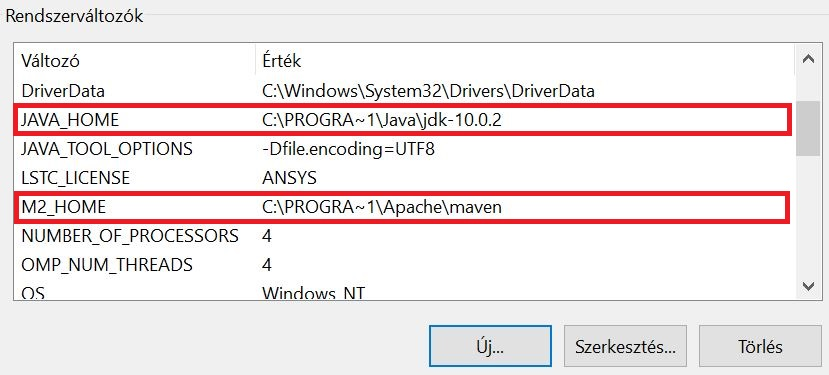
\includegraphics{env-variable}
\caption{Szükséges környezeti változók beállítása}
\label{fig:envvar}
\end{figure}

\begin{figure}[h]
\centering
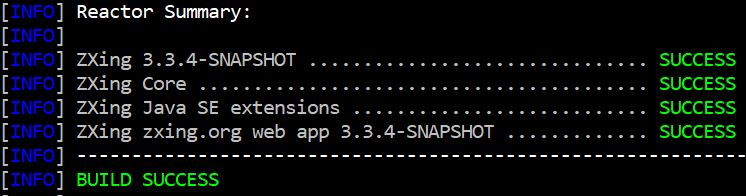
\includegraphics{zxingbuild}
\caption{Sikeres build végeredménye}
\label{fig:buildsuccess}
\end{figure}

A lefordított .jar fájlokat ezt követően az egyes modulokon belül találjuk. Például a lefordított \textit{core/} kód helye a \textit{core/target/core-x.y.z.jar}. Ezeket lehet beimportálni a képfeldolgozást megvalósító projektbe.

\subsubsection{ZXing könyvtár beimportálása és használata}
Az iiwa robotkart programozni Sunrise Workbench használatával a legegyszerűbb, ami egy JAVA Eclipse platformú szoftver. Emiatt praktikus okokból a szakdolgozat képfeldolgozási és sakkalgoritmus beágyazási része túlnyomó részt Eclipse-ben történt (verzió: 4.9.0)\footnote{Link: https://www.eclipse.org/}.

A könyvtár beimportálásához létrehoztam egy java projektet. Erre jobb egérgombbal kattintva elnavigáltam a `\angol{Configure Build Path...}' menüponthoz (\ref{fig:zxingimport}. ábra). A `\angol{Classpath}'-t kiválasztva jobb oldalt aktivizálódik az `\angol{Add External Jars...}' gomb. Kiválasztottam a \textit{core/} és a \textit{javase/} modulok .jar fájljait. Ezeken belül lehetőség van forráskód (\angol{Source attachment}) és dokumentáció (\angol{Javadoc location}) csatolására (\ref{fig:zxingimport}. ábra). `\angol{Apply and Close}' után megjelennek a csomagok a hivatkozott könyvtárak (\angol{Referenced libraries}) pont alatt.

\begin{figure}[h]
\centering
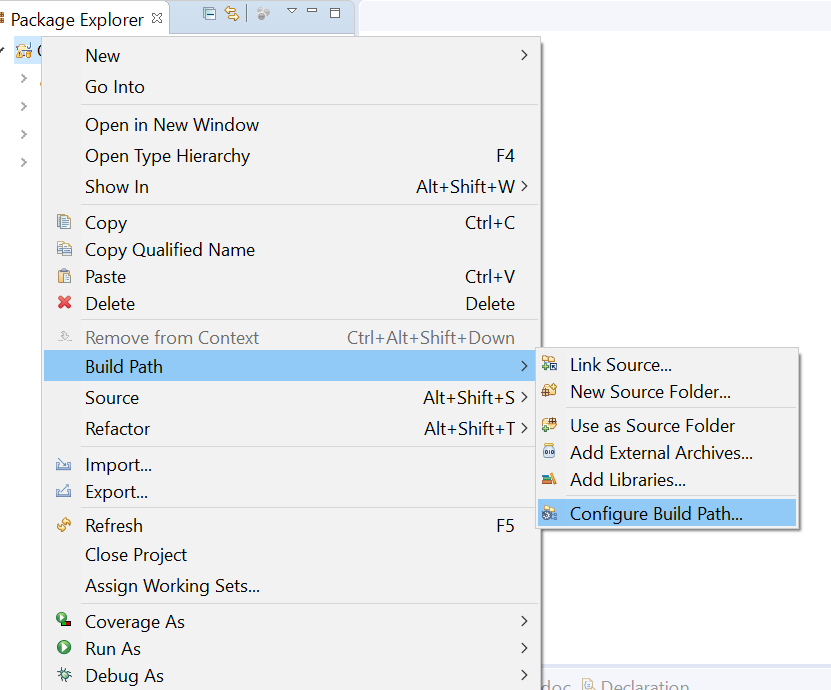
\includegraphics[scale=0.5]{buildpath}
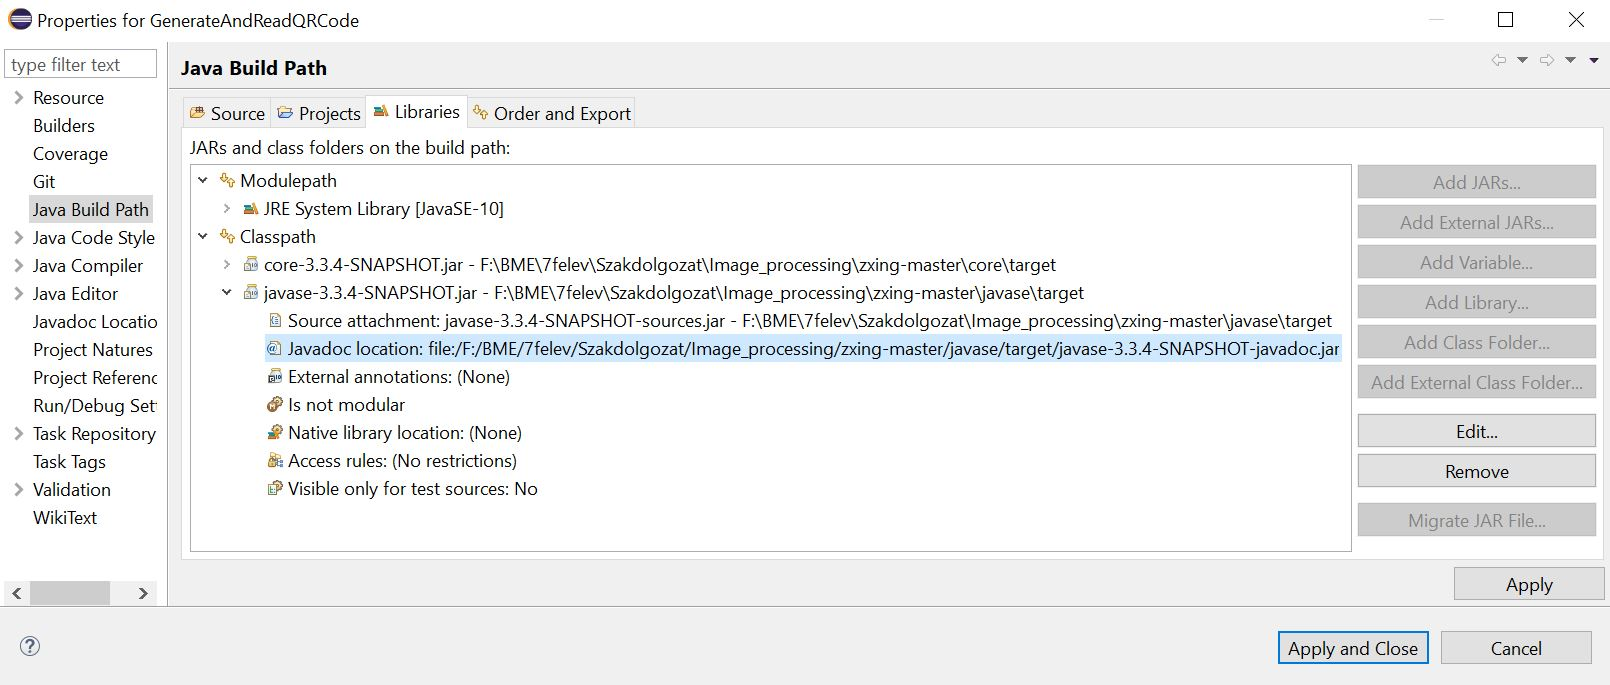
\includegraphics[scale=0.5]{zxingimport}
\caption{ZXing hozzáadása a hivatkozott könyvtárakhoz}
\label{fig:zxingimport}
\end{figure}

\subsubsection{QR kód generálás és olvasás}
A ZXing könyvtárt felhasználó, ehhez a projekthez szükséges elemek az `imgprocess' csomagban találhatóak a `QRCodeMethods.java' fájlban. A függvények leírása  \aref{tab:qrcodemethods} táblázatban találhatóak\footnote{Forráskód: https://github.com/rolandvarga601/Szakdolgozat}. 

\begin{table}[h]
\centering
\renewcommand\tabularxcolumn[1]{m{#1}}% for vertical centering text in X column
\begin{tabularx}{\linewidth}{|c|X|X|}
\hline \multicolumn{1}{|c|}{\textbf{Függvény neve}} & \multicolumn{1}{c|}{\textbf{Paraméterek}} & \multicolumn{1}{c|}{\textbf{Leírás}}\tabularnewline \hline
createQRCode & 
\begin{itemize} \item String qrCodeData - a kódolt szöveg
					\item String filePath - a képek mentési helye
					\item String charset - karakterkódolás
					\item int qrCodeheight - a kép magassága
					\item int qrCodewidth - a kép szélessége
\end{itemize} & Nincs visszatérési értéke, a QR-kódot tartalmazó képet a megadott elérési helyre menti. \tabularnewline \hline
readQRCode & BufferedImage image - a kép amelyen a QR-kód található & Visszaadja a képen található QR-kódba kódolt szöveget. \tabularnewline \hline
readMultiQRCode & String FileName - a kép elérési útja, amelyen a QR-kódok találhatóak & Képes egyazon képen különböző szögekben elhelyezkedő QR-kódok felismerésére és dekódolására (\ref{fig:multiqrcoderead} ábra). Visszatérési érték: Result[], amely tömb elemei tartalmazzák többek között az egyes QR-kódok helyét a képeken és a kódolt szöveget. \tabularnewline \hline
\end{tabularx}
\caption{QRCodeMethods.java függvényei}
\label{tab:qrcodemethods}
\end{table}

\begin{figure}[h]
\centering
\fbox{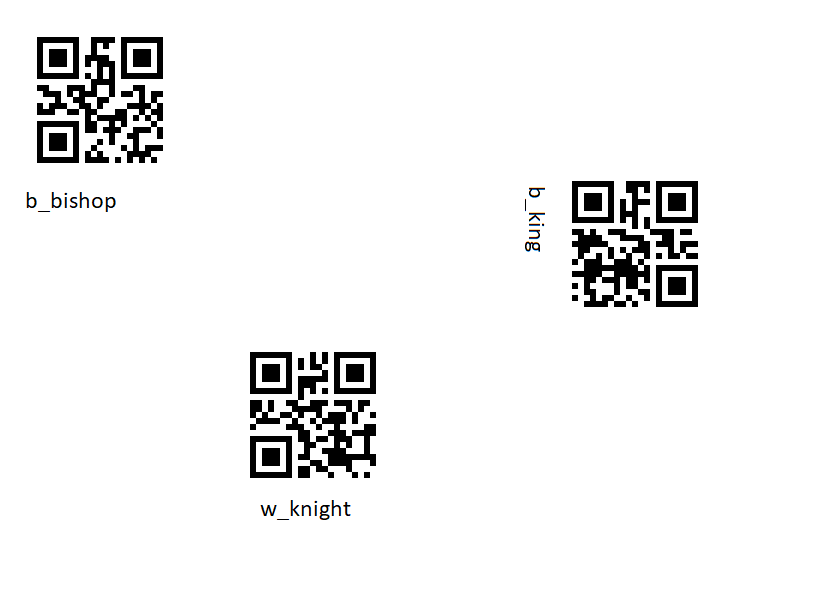
\includegraphics[scale=0.5]{multiqrcode}}
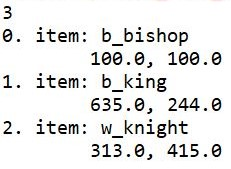
\includegraphics[scale=0.8]{multiqrcoderesult}
\caption{Példa a több QR-kódot tartalmazó kép kiolvasására}
\label{fig:multiqrcoderead}
\end{figure}

















\end{document}